\section{Progettazione logica}

\subsection{Analisi delle ridondanze}
Nello schema concettuale possiamo individuare stato di occupazione che è attributo di molo e deducibile dalla relazione sosta, la quale presenta l'attributo data di arrivo e data di partenza.

Le operazioni coinvolte sono la numero 3 e la numero 6 che presentano una frequenza di 40 volte al giorno e 30-40 volte ogni giorno.

Si procede alla valutazione del costo totale in termini di accessi nel caso di ridondanza e di assenza di essa.

\begin{center}
    \begin{tabularx}{\textwidth}{|p{90mm}|X|}
        \hline
        \rowcolor{gray!30}
        \textbf{Operazione} & \textbf{Frequenza}\\
        \hline
        3. Controllo dei posti disponibili per una certa imbarcazione(Controllo delle dimensioni)& 40 volte al giorno\\
        \hline
        6. Arrivo di un'imbarcazione nel marina & 30-40 volte al giorno\\
        \hline
    \end{tabularx}
\end{center}

Ci riferiremo per i nostri calcoli a dei volumi plausibili nella vita della base di dati. I moli non variano particolarmente di numero, le imbarcazioni vengono registrate al loro primo accesso e le soste aumentano ogni giorno. Mediamente un'imbarcazione sosta 2,7 volte in un molo.

\begin{center}
    \begin{tabularx}{\textwidth}{|X|X|X|}
        \hline
        \rowcolor{gray!30}
        \textbf{Concetto} & \textbf{Tipo} & \textbf{Volume}\\
        \hline
        Molo & ENTITÀ & 250\\
        \hline
        Imbarcazione & ENTITÀ & 5000\\
        \hline
        Sosta & ENTITÀ & 13500\\ % Contando che ogni imbarcazione sosta in media due volte per molo.
        \hline
        M\_S & RELAZIONE & 13500\\ % Contando che ogni imbarcazione sosta in media due volte per molo.
        \hline
    \end{tabularx}
\end{center}

\paragraph{operazione 3}

\begin{center}
    \begin{minipage}{.48\linewidth}
        \begin{tabularx}{\linewidth}{|X|l|l|l|}
            \hline
            \rowcolor{gray!30}
            \multicolumn{4}{|c|}{\textbf{Con ridondanza}}\\
            \hline
            \rowcolor{gray!15}
            Concetto & Costrutto & Accessi & Tipo\\
            \hline
            Molo & E & 250 & L\\
            \hline
        \end{tabularx}
    \end{minipage}
    \begin{minipage}{.48\linewidth}
        \begin{tabularx}{\linewidth}{|X|l|l|l|}
            \hline
            \rowcolor{gray!30}
            \multicolumn{4}{|c|}{\textbf{Senza ridondanza}}\\
            \hline
            \rowcolor{gray!15}
            Concetto & Costrutto & Accessi & Tipo\\
            \hline
            Sosta & E & 13500 & L\\
            \hline
            M\_S & R & 13500 & L\\
            \hline
            Molo & E & 250 & L\\
            \hline
        \end{tabularx}
    \end{minipage}
\end{center}

\underline{Con ridondanza}
\begin{itemize}
    \item Totale accessi(Solo in lettura): $250\xrightarrow{*40} 10000$
\end{itemize}

\underline{Senza ridondanza}
\begin{itemize}
    \item Totale accessi(Solo in lettura): $250+13500+13500 = 27250 \xrightarrow{*40} 1090000$ Giornalieri
\end{itemize}

\paragraph{operazione 6}

Assumo che l'imbarcazione sia già presente perché l'esserci o non esserci non cambia il calcolo della ridondanza.

\begin{center}
\begin{tabularx}{\linewidth}{|X|}
    \hline
    \rowcolor{gray!30}
    \multicolumn{1}{|c|}{\textbf{Operazioni principali}}\\
    \hline
    Cerco l'imbarcazione\\
    \hline
    Cerco i moli disponibili\\
    \hline
    Confronto le dimensioni dell'imbarcazione con i moli disponibili\\
    \hline
    Scrivo la sosta\\
    \hline
\end{tabularx}
\end{center}


\begin{center}
    \begin{minipage}{.48\linewidth}
        \begin{tabularx}{\linewidth}{|X|l|l|l|}
            \hline
            \rowcolor{gray!30}
            \multicolumn{4}{|c|}{\textbf{Con ridondanza}}\\
            \hline
            \rowcolor{gray!15}
            Concetto & Costrutto & Accessi & Tipo\\
            \hline
            Imbarcazione & E & 1 & L\\
            \hline
            Molo & E & 250 & L\\
            \hline
            Sosta & E & 1 & S\\
            \hline
            Molo & E & 1 & S\\
            \hline
        \end{tabularx}
    \end{minipage}
    \begin{minipage}{.48\linewidth}
        \begin{tabularx}{\linewidth}{|X|l|l|l|}
            \hline
            \rowcolor{gray!30}
            \multicolumn{4}{|c|}{\textbf{Senza ridondanza}}\\
            \hline
            \rowcolor{gray!15}
            Concetto & Costrutto & Accessi & Tipo\\
            \hline
            Imbarcazione & E & 1 & L\\
            \hline
            Sosta & E & 13500 & L\\
            \hline
            M\_S & R & 13500 & L\\
            \hline
            Molo & E & 250 & L\\
            \hline
            Sosta & E & 1 & S\\
            \hline
        \end{tabularx}
    \end{minipage}
\end{center}


\underline{Con ridondanza}
\begin{itemize}
    \item Totale scritture: $1 + 1 = 2 \xrightarrow{*2} 4$ 
    \item Totale letture: $250 + 1 = 251$
    \item Totale accessi: $4+251 = 255 \xrightarrow{*40} 102000$ Giornalieri
\end{itemize}
\underline{Senza ridondanza}
\begin{itemize}
    \item Totale scritture: $1 \xrightarrow{*2} 2$ 
    \item Totale letture: $1 + 13500 + 13500 + 250 = 27251$
    \item Totale accessi: $2+27251 = 27253 \xrightarrow{*40} 1090120$ Giornalieri
\end{itemize}

\paragraph{In conclusione}
Nell'\textbf{operazione 2} e nell'\textbf{operazione 6} risulta meno costosa in termini di accessi l'operazione con ridondanza. Notando un grosso divario tra le operazioni con ridondanza e le operazioni senza ridondanza, qui si sceglie di mantenere la ridondanza diminuendo il numero di accessi necessari.

\subsubsection{altre ridondanze}

Un altra ridondanza è Quantità di soste in \textbf{Cliente occasionale} è deducibile da Cliente possiede imbarcazione che sosta in un molo andando a vedere quante soste hanno effettuato le sue imbarcazioni;

In seguito all'analisi sugli accessi abbiamo stimato che risulti essere preferibile mantenere la ridondanza relativamente ad eventuali operazioni di lettura e scrittura di questi valori, 
pertanto si è deciso di mantenere la ridondanza.


\subsection{Eliminazione degli attributi multi-valore}

Contatto in Persona è multi-valore.

Abbiamo quindi reificato contatto in una relazione binaria come segue.

\begin{center}
    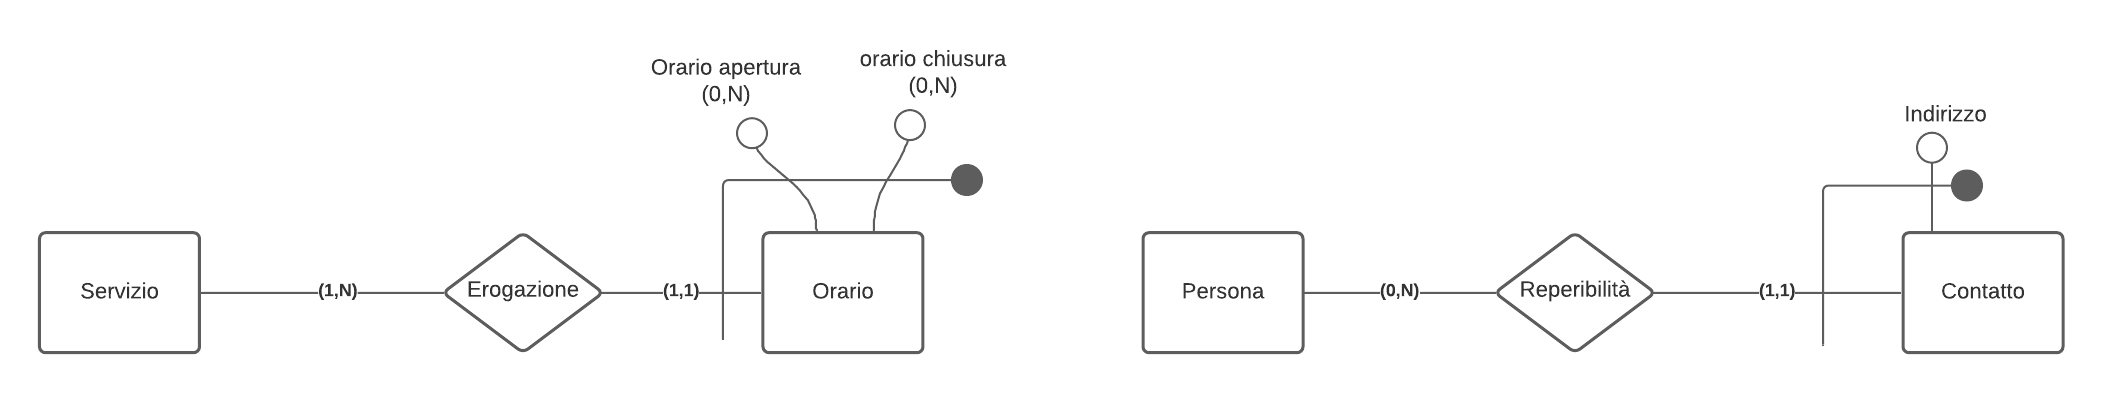
\includegraphics[width=\linewidth / 2]{img/multi_valore.png}
\end{center}


\subsection{Eliminazione delle generalizzazioni}

\paragraph{Cliente}\mbox{}\\
Si accorpano Cliente abituale e cliente occasionale a Cliente. Dato che la quantità di soste è un attributo utile per entrambe le tipologie di cliente. Lo sconto personale sarà invece impostato ad un valore che indica la percentuale di sconto se il cliente è abituale e a NULL se il cliente è occasionale.

\paragraph{Persona}\mbox{}\\
Nelle generalizzazioni di persona, per evitare inutili valori NULL in un eventuale accorpamento \textbf{Persona} viene mantenuta come entità. Questa entità conterrà tutti i dati relativi alla persona e avrà due entità deboli collegate ovvero \textbf{Addetto} e \textbf{Cliente}.

Persona avrà da 0 a 1 \textbf{Cliente} e da 0 a 1 \textbf{Addetto}. Chiaramente ogni \textbf{Cliente}  e \textbf{Addetto} avrà una e una sola persona legata. In \textbf{Addetto} e \textbf{Cliente} posizioneremo i dati relativi a queste due entità come da schema concettuale.

\subsection{Modifiche, aggiunte e chiarimenti alle chiavi}

Tutte le chiavi primarie sono definite utilizzando le chiavi della progettazione concettuale, tranne nei seguenti casi.

\paragraph{Imbarcazione} Ad \textbf{Imbarcazione} oltre alla sua chiave primaria Codice internazionale viene aggiunto un id autoincrementante utilizzato come chiave\footnote{Chiave unica}. Questo è stato scelto per poter utilizzare il costraint relativo alla sovrapposizione delle soste. Infatti esso funziona solo con attributi interi e non con Varchar\footnote{A meno di installare il pacchetto aggiuntivo di Postgres che lo permetta ma per lo scopo di questo progetto abbiamo preferito evitare per questioni di compatibilità.}.

\paragraph{Cliente} A \textbf{Cliente} oltre alla sua chiave primaria \textit{Codice fiscale} viene aggiunto un id autoincrementante utilizzato come chiave\footnote{Chiave unica}. Questo è stato scelto per poter utilizzare il costraint relativo alla sovrapposizione delle prenotazioni. Infatti esso funziona solo con attributi interi e non con Varchar.

\paragraph{Addetto} Addetto concettualmente eredita la chiave primaria di \textbf{Persona} ma come da progettazione concettuale mantiene la chiave su \underline{Servizio gestito, Data inizio contratto}. Come chiave primaria si sceglie quindi di utilizzare il \textit{codice fiscale} derivante da \textbf{persona} perché più leggero.

\paragraph{Periodo di apertura} Per ridurre lo spazio utilizzato nella tabella che rappresenta la relazione \textit{Apertura}, a \textbf{Periodo di apertura} abbiamo aggiunto una chiave primaria tramite id autoincrementante. Chiaramente non abbiamo rimosso la chiave unica già presente, infatti essa garantisce l'unicità delle triple presenti.

\paragraph{Sosta} Per semplificare il lavoro con le prenotazioni trasformate in \textbf{Sosta} a sosta viene aggiunto un id autoincrementante come chiave. Questo id verrà utilizzato da \textbf{Prenotazione} per definire se la prenotazione è stata trasformata in sosta.


\subsection{Schema concettuale ristrutturato - Schema logico}
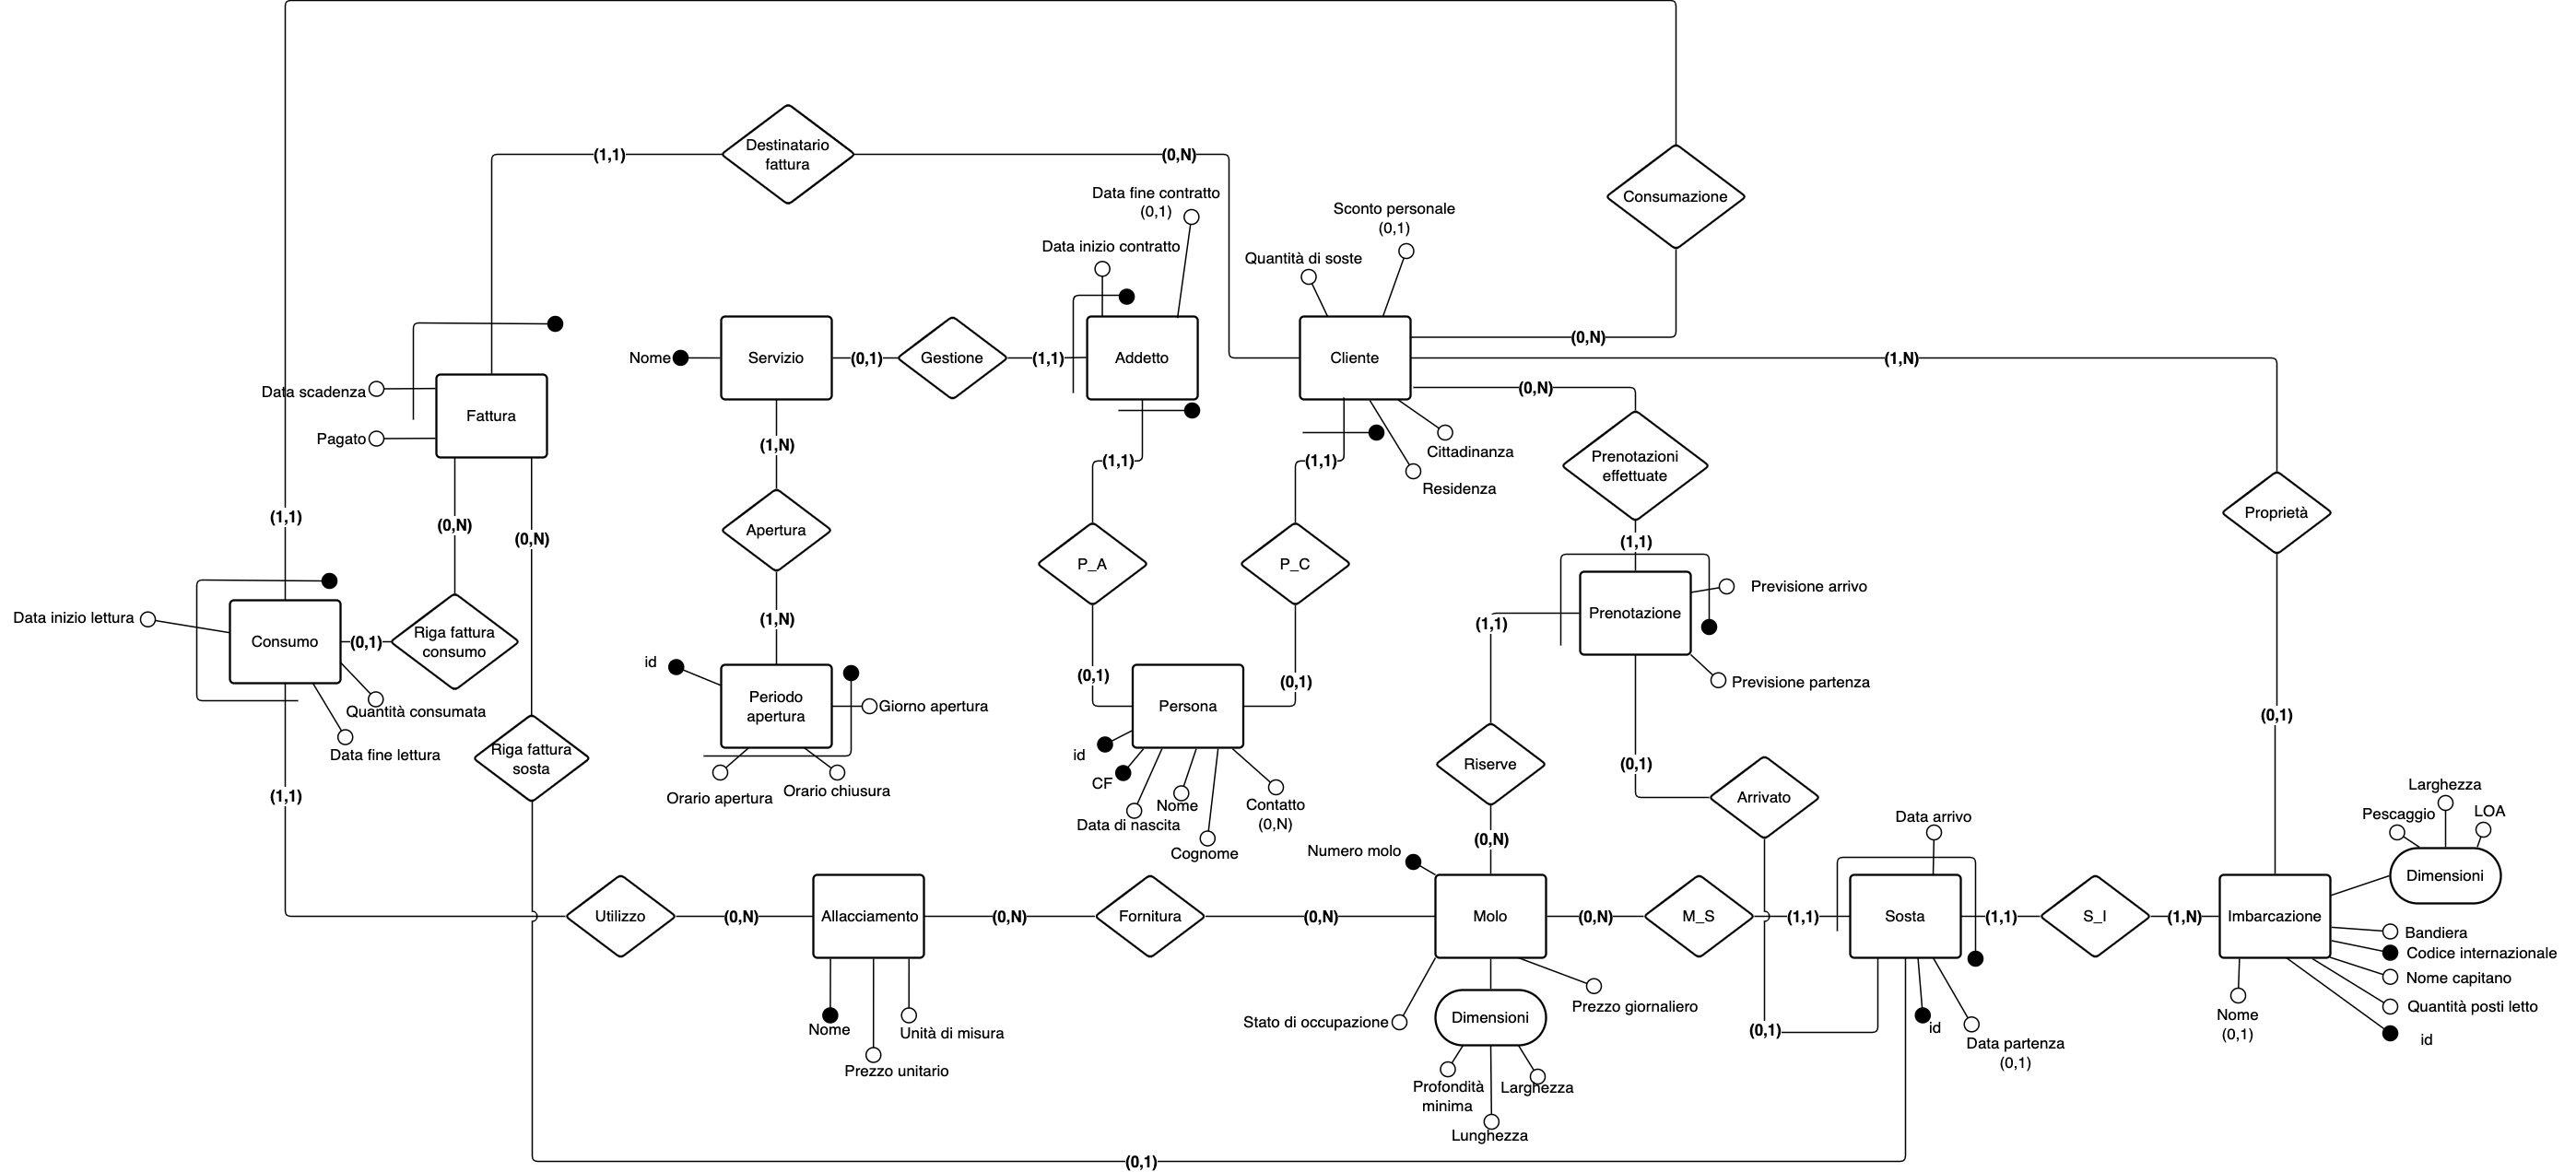
\includegraphics[width=\textwidth]{img/erlogico.png}


\subsection{Descrizione schema relazionale}

Per questione di compatibilità con il \textit{DBMS} alcuni nomi di attributi entità e relazioni sono stati normalizzati, utilizzando il camelCase, togliendo gli accenti, accorciando i nomi molto lunghi e con altre piccole accortezze.\\

\textbf{Imbarcazione}(\underline{\textit{codiceInternazionale}}, \underline{id}, cliente, bandiera, nomeCapitano, nPostiLetto, nome, pescaggio, larghezza, LOA);

\textbf{Molo} (\underline{\textit{id}}, occupato, profonditaMinima, larghezza, lunghezza, prezzoGiorno);

\textbf{Servizio} (\underline{\textit{nome}});

\textbf{Addetto} (\underline{\textit{persona}}, \underline{servizio, inizioContratto}, fineContratto);

\textbf{Cliente} (\underline{\textit{persona}}, \underline{id}, cittadinanza, residenza, quantitaSoste, scontoPersonale);

\textbf{Persona} (\underline{\textit{CF}}, dataNascita, nome, cognome);

\textbf{Prenotazione} (\underline{\textit{cliente, prevArrivo, molo}}, prevPartenza, sosta);

\textbf{Sosta} (\underline{\textit{imbarcazione, molo, arrivo}}, \underline{id}, partenza, fattura);

\textbf{Allacciamento} (\underline{\textit{nome}}, prezzoUnitario, unitaMisura);

\textbf{Fornitura} (\underline{\textit{allacciamento, molo}});

\textbf{PeriodoApertura} (\underline{\textit{id}}, \underline{giorno, apertura, chiusura});

\textbf{AperturaServizio} (\underline{\textit{servizio, periodoApertura}});

\textbf{Consumo}(\underline{\textit{cliente, allaciamento, inizio}}, fine, quantita, fattura);

\textbf{Fattura}(\underline{\textit{id}},\underline{cliente, scadenza}, pagato);\\

La chiave primaria è la prima delle chiavi indicate dalla sottilineatura.

\subsection{Vincoli di integrità referenziali}

\textbf{Imbarcazione}.cliente -> \textit{Cliente}.persona\\
\textbf{Addetto}.persona -> \textit{Persona}.CF\\
\textbf{Cliente}.persona -> \textit{Persona}.CF\\
\textbf{Prenotazione}.cliente -> \textit{Cliente}.id\\
\textbf{Prenotazione}.molo -> \textit{Molo}.id\\
\textbf{Prenotazione}.sosta -> \textit{Sosta}.id\\
\textbf{Sosta}.imbarcazione -> \textit{Imbarcazione}.id\\
\textbf{Sosta}.molo -> \textit{Molo}.id\\
\textbf{Sosta}.fattura -> \textit{Fattura}.id\\
\textbf{Fornitura}.allacciamento -> \textit{Allacciamento}.nome\\
\textbf{Fornitura}.molo -> \textit{Molo}.id\\
\textbf{AperturaServizio}.servizio -> \textit{Servizio}.nome\\
\textbf{AperturaServizio}.periodoApertura -> \textit{PeriodoApertura}.id\\
\textbf{Consumo}.cliente -> \textit{Cliente}.persona\\
\textbf{Consumo}.allacciamento -> \textit{Allacciamento}.nome\\
\textbf{Consumo}.fattura -> \textit{Fattura}.id\\
\textbf{Fattura}.cliente -> \textit{Cliente}.persona\\

\subsection{Check e costraint}

\subsubsection{Vincoli non gestiti}
Non è stato purtroppo possibile mantenere fede a tutti i vincoli posti nella progettazione concettuale, e relativamente ad essi viene lasciato al programmatore che utilizzerà la base dati l'onere di mantenerla consistente.

\paragraph{Fattura}
Non viene quindi gestito il vincolo relativo a fattura, per via di una dipendenza circolare tra la generazione della fattura e la creazione delle sue linee. Si considera quindi la fattura con zero linee come "\textit{fattura da riempire}".

\paragraph{Molo}
Per gestire la consistenza di \textbf{Molo} si possono utilizzare dei trigger che la controllino ad ogni variazione dei dati. Ma per ridurre la complessità si è deciso anche qui di lasciare l'onere della consistenza al programmatore.

\subsubsection{Vincoli gestiti}

\paragraph{PeriodoApertura}
In \textbf{PeriodoApertura} è attivato un check che controlla che l'orario di chiusura sia sempre postumo all'orario di apertura.

\paragraph{Prenotazione e Sosta}
In \textbf{Prenotazione} ed in \textbf{Sosta} viene eseguito un check simile a quello di \textbf{PeriodoApertura}. In queste due entità viene quindi controllato che il momento della partenza sia sempre postumo al momento dell'arrivo, questo anche quando la partenza è non definita. Per fare questo si è quindi deciso di settare la partenza con valore di default ad "\textit{infinito}" in sosta.

In queste due entità vengono inoltre fatti due controlli relativi alla sovrapposizione di soste e prenotazioni.

Se un \textbf{Molo} è già occupato in un determinato periodo esso non sarà occupabile, e se un'\textbf{Imbarcazione} si trova già in un \textbf{Molo} non potrà sdoppiarsi ed essere sostante in più moli contemporaneamente.

Come precedentemente accennato per implementare questo costraint sono state fatte delle modifiche alle chiavi di imbarcazione e di cliente, aggiungendo una chiave intera in modo da poter utilizzare i GIST\footnote{Generalized Search Tree, ovvero un albero di ricerca molto simile al B-Tree} nella versione standard di Postgres\footnote{DBMS scelto per il progetto presente}.

